% Options for packages loaded elsewhere
% Options for packages loaded elsewhere
\PassOptionsToPackage{unicode}{hyperref}
\PassOptionsToPackage{hyphens}{url}
\PassOptionsToPackage{dvipsnames,svgnames,x11names}{xcolor}
%
\documentclass[
  spanish,
  a4paper,
  oneside]{scrbook}
\usepackage{xcolor}
\usepackage[top=25mm,bottom=25mm,left=30mm,right=20mm]{geometry}
\usepackage{amsmath,amssymb}
\setcounter{secnumdepth}{-\maxdimen} % remove section numbering
\usepackage{iftex}
\ifPDFTeX
  \usepackage[T1]{fontenc}
  \usepackage[utf8]{inputenc}
  \usepackage{textcomp} % provide euro and other symbols
\else % if luatex or xetex
  \usepackage{unicode-math} % this also loads fontspec
  \defaultfontfeatures{Scale=MatchLowercase}
  \defaultfontfeatures[\rmfamily]{Ligatures=TeX,Scale=1}
\fi
\usepackage{lmodern}
\ifPDFTeX\else
  % xetex/luatex font selection
\fi
% Use upquote if available, for straight quotes in verbatim environments
\IfFileExists{upquote.sty}{\usepackage{upquote}}{}
\IfFileExists{microtype.sty}{% use microtype if available
  \usepackage[]{microtype}
  \UseMicrotypeSet[protrusion]{basicmath} % disable protrusion for tt fonts
}{}
\makeatletter
\@ifundefined{KOMAClassName}{% if non-KOMA class
  \IfFileExists{parskip.sty}{%
    \usepackage{parskip}
  }{% else
    \setlength{\parindent}{0pt}
    \setlength{\parskip}{6pt plus 2pt minus 1pt}}
}{% if KOMA class
  \KOMAoptions{parskip=half}}
\makeatother
% Make \paragraph and \subparagraph free-standing
\makeatletter
\ifx\paragraph\undefined\else
  \let\oldparagraph\paragraph
  \renewcommand{\paragraph}{
    \@ifstar
      \xxxParagraphStar
      \xxxParagraphNoStar
  }
  \newcommand{\xxxParagraphStar}[1]{\oldparagraph*{#1}\mbox{}}
  \newcommand{\xxxParagraphNoStar}[1]{\oldparagraph{#1}\mbox{}}
\fi
\ifx\subparagraph\undefined\else
  \let\oldsubparagraph\subparagraph
  \renewcommand{\subparagraph}{
    \@ifstar
      \xxxSubParagraphStar
      \xxxSubParagraphNoStar
  }
  \newcommand{\xxxSubParagraphStar}[1]{\oldsubparagraph*{#1}\mbox{}}
  \newcommand{\xxxSubParagraphNoStar}[1]{\oldsubparagraph{#1}\mbox{}}
\fi
\makeatother

\usepackage{color}
\usepackage{fancyvrb}
\newcommand{\VerbBar}{|}
\newcommand{\VERB}{\Verb[commandchars=\\\{\}]}
\DefineVerbatimEnvironment{Highlighting}{Verbatim}{commandchars=\\\{\}}
% Add ',fontsize=\small' for more characters per line
\usepackage{framed}
\definecolor{shadecolor}{RGB}{241,243,245}
\newenvironment{Shaded}{\begin{snugshade}}{\end{snugshade}}
\newcommand{\AlertTok}[1]{\textcolor[rgb]{0.68,0.00,0.00}{#1}}
\newcommand{\AnnotationTok}[1]{\textcolor[rgb]{0.37,0.37,0.37}{#1}}
\newcommand{\AttributeTok}[1]{\textcolor[rgb]{0.40,0.45,0.13}{#1}}
\newcommand{\BaseNTok}[1]{\textcolor[rgb]{0.68,0.00,0.00}{#1}}
\newcommand{\BuiltInTok}[1]{\textcolor[rgb]{0.00,0.23,0.31}{#1}}
\newcommand{\CharTok}[1]{\textcolor[rgb]{0.13,0.47,0.30}{#1}}
\newcommand{\CommentTok}[1]{\textcolor[rgb]{0.37,0.37,0.37}{#1}}
\newcommand{\CommentVarTok}[1]{\textcolor[rgb]{0.37,0.37,0.37}{\textit{#1}}}
\newcommand{\ConstantTok}[1]{\textcolor[rgb]{0.56,0.35,0.01}{#1}}
\newcommand{\ControlFlowTok}[1]{\textcolor[rgb]{0.00,0.23,0.31}{\textbf{#1}}}
\newcommand{\DataTypeTok}[1]{\textcolor[rgb]{0.68,0.00,0.00}{#1}}
\newcommand{\DecValTok}[1]{\textcolor[rgb]{0.68,0.00,0.00}{#1}}
\newcommand{\DocumentationTok}[1]{\textcolor[rgb]{0.37,0.37,0.37}{\textit{#1}}}
\newcommand{\ErrorTok}[1]{\textcolor[rgb]{0.68,0.00,0.00}{#1}}
\newcommand{\ExtensionTok}[1]{\textcolor[rgb]{0.00,0.23,0.31}{#1}}
\newcommand{\FloatTok}[1]{\textcolor[rgb]{0.68,0.00,0.00}{#1}}
\newcommand{\FunctionTok}[1]{\textcolor[rgb]{0.28,0.35,0.67}{#1}}
\newcommand{\ImportTok}[1]{\textcolor[rgb]{0.00,0.46,0.62}{#1}}
\newcommand{\InformationTok}[1]{\textcolor[rgb]{0.37,0.37,0.37}{#1}}
\newcommand{\KeywordTok}[1]{\textcolor[rgb]{0.00,0.23,0.31}{\textbf{#1}}}
\newcommand{\NormalTok}[1]{\textcolor[rgb]{0.00,0.23,0.31}{#1}}
\newcommand{\OperatorTok}[1]{\textcolor[rgb]{0.37,0.37,0.37}{#1}}
\newcommand{\OtherTok}[1]{\textcolor[rgb]{0.00,0.23,0.31}{#1}}
\newcommand{\PreprocessorTok}[1]{\textcolor[rgb]{0.68,0.00,0.00}{#1}}
\newcommand{\RegionMarkerTok}[1]{\textcolor[rgb]{0.00,0.23,0.31}{#1}}
\newcommand{\SpecialCharTok}[1]{\textcolor[rgb]{0.37,0.37,0.37}{#1}}
\newcommand{\SpecialStringTok}[1]{\textcolor[rgb]{0.13,0.47,0.30}{#1}}
\newcommand{\StringTok}[1]{\textcolor[rgb]{0.13,0.47,0.30}{#1}}
\newcommand{\VariableTok}[1]{\textcolor[rgb]{0.07,0.07,0.07}{#1}}
\newcommand{\VerbatimStringTok}[1]{\textcolor[rgb]{0.13,0.47,0.30}{#1}}
\newcommand{\WarningTok}[1]{\textcolor[rgb]{0.37,0.37,0.37}{\textit{#1}}}

\usepackage{longtable,booktabs,array}
\usepackage{calc} % for calculating minipage widths
% Correct order of tables after \paragraph or \subparagraph
\usepackage{etoolbox}
\makeatletter
\patchcmd\longtable{\par}{\if@noskipsec\mbox{}\fi\par}{}{}
\makeatother
% Allow footnotes in longtable head/foot
\IfFileExists{footnotehyper.sty}{\usepackage{footnotehyper}}{\usepackage{footnote}}
\makesavenoteenv{longtable}
\usepackage{graphicx}
\makeatletter
\newsavebox\pandoc@box
\newcommand*\pandocbounded[1]{% scales image to fit in text height/width
  \sbox\pandoc@box{#1}%
  \Gscale@div\@tempa{\textheight}{\dimexpr\ht\pandoc@box+\dp\pandoc@box\relax}%
  \Gscale@div\@tempb{\linewidth}{\wd\pandoc@box}%
  \ifdim\@tempb\p@<\@tempa\p@\let\@tempa\@tempb\fi% select the smaller of both
  \ifdim\@tempa\p@<\p@\scalebox{\@tempa}{\usebox\pandoc@box}%
  \else\usebox{\pandoc@box}%
  \fi%
}
% Set default figure placement to htbp
\def\fps@figure{htbp}
\makeatother


% definitions for citeproc citations
\NewDocumentCommand\citeproctext{}{}
\NewDocumentCommand\citeproc{mm}{%
  \begingroup\def\citeproctext{#2}\cite{#1}\endgroup}
\makeatletter
 % allow citations to break across lines
 \let\@cite@ofmt\@firstofone
 % avoid brackets around text for \cite:
 \def\@biblabel#1{}
 \def\@cite#1#2{{#1\if@tempswa , #2\fi}}
\makeatother
\newlength{\cslhangindent}
\setlength{\cslhangindent}{1.5em}
\newlength{\csllabelwidth}
\setlength{\csllabelwidth}{3em}
\newenvironment{CSLReferences}[2] % #1 hanging-indent, #2 entry-spacing
 {\begin{list}{}{%
  \setlength{\itemindent}{0pt}
  \setlength{\leftmargin}{0pt}
  \setlength{\parsep}{0pt}
  % turn on hanging indent if param 1 is 1
  \ifodd #1
   \setlength{\leftmargin}{\cslhangindent}
   \setlength{\itemindent}{-1\cslhangindent}
  \fi
  % set entry spacing
  \setlength{\itemsep}{#2\baselineskip}}}
 {\end{list}}
\usepackage{calc}
\newcommand{\CSLBlock}[1]{\hfill\break\parbox[t]{\linewidth}{\strut\ignorespaces#1\strut}}
\newcommand{\CSLLeftMargin}[1]{\parbox[t]{\csllabelwidth}{\strut#1\strut}}
\newcommand{\CSLRightInline}[1]{\parbox[t]{\linewidth - \csllabelwidth}{\strut#1\strut}}
\newcommand{\CSLIndent}[1]{\hspace{\cslhangindent}#1}

\ifLuaTeX
\usepackage[bidi=basic]{babel}
\else
\usepackage[bidi=default]{babel}
\fi
% get rid of language-specific shorthands (see #6817):
\let\LanguageShortHands\languageshorthands
\def\languageshorthands#1{}


\setlength{\emergencystretch}{3em} % prevent overfull lines

\providecommand{\tightlist}{%
  \setlength{\itemsep}{0pt}\setlength{\parskip}{0pt}}



 


\AtBeginDocument{\hypersetup{linkcolor=black}}
% ---------- Paquetes tipograficos y microajustes ----------
\usepackage{microtype}        % mejor interletrado y justificado
\usepackage{csquotes}         % comillas tipograficas
\usepackage{iftex}
\ifPDFTeX\else
  % Seleccion de fuentes solo cuando XeTeX/LuaTeX esta disponible.
  \IfFontExistsTF{TeX Gyre Termes}{
    \setmainfont{TeX Gyre Termes}
  }{
    \IfFontExistsTF{Latin Modern Roman}{\setmainfont{Latin Modern Roman}}{}
  }
  \IfFontExistsTF{TeX Gyre Heros}{
    \setsansfont{TeX Gyre Heros}
  }{
    \IfFontExistsTF{Latin Modern Sans}{\setsansfont{Latin Modern Sans}}{}
  }
  \IfFontExistsTF{TeX Gyre Cursor}{
    \setmonofont{TeX Gyre Cursor}
  }{
    \IfFontExistsTF{Latin Modern Mono}{\setmonofont{Latin Modern Mono}}{}
  }
\fi
\usepackage{enumitem}         % listas compactas
\setlist{itemsep=.2em, topsep=.2em}

% ---------- KOMA-Script: estilo de titulos y espaciado ----------
\KOMAoptions{
  headings=big,
  parskip=half,
  fontsize=12pt,
  appendixprefix=true
}
\setlength{\parindent}{1.5em}
\setlength{\parskip}{0.6em}
\usepackage{indentfirst}
\usepackage{setspace}         % Control del interlineado del documento
\setstretch{1.5}

% ---------- Encabezados y pies (scrlayer-scrpage) ----------
\usepackage[automark,headsepline]{scrlayer-scrpage}
\clearpairofpagestyles
\automark[chapter]{chapter}
\ihead{\pagemark}
\ohead{\itshape\headmark}
\setheadsepline{0.4pt}
\renewcommand*{\chaptermarkformat}{}
\renewcommand*{\chapterpagestyle}{scrheadings}
\pagestyle{scrheadings}
\makeatletter
\let\ps@plain\ps@scrheadings
\makeatother
\cfoot{}

% ---------- Hipervinculos mas sobrios ----------
\usepackage{hyperref}
\hypersetup{
  colorlinks=true,
  linkcolor=black,
  citecolor=[rgb]{0.05,0.2,0.5},
  urlcolor=[rgb]{0.05,0.2,0.5},
  pdfauthor={\@author},
  pdftitle={\@title}
}

% ---------- Leyendas de figuras/tablas ----------
\usepackage[labelfont=bf,textfont=it]{caption}
\captionsetup{
  skip=8pt
}

% ---------- Tabla de contenidos ----------
\KOMAoptions{toc=graduated}
\RedeclareSectionCommand[tocnumwidth=3em]{chapter}
\RedeclareSectionCommand[tocindent=3.25em,tocnumwidth=2.8em]{section}
\RedeclareSectionCommand[tocindent=6.5em,tocnumwidth=2.5em]{subsection}
\makeatletter
\newcommand*{\tocdotfill}{\leavevmode\leaders\hbox to .6em{\hss.\hss}\hfill}
\makeatother
\RedeclareSectionCommand[toclinefill=\tocdotfill]{chapter}
\RedeclareSectionCommand[toclinefill=\tocdotfill]{section}
\RedeclareSectionCommand[toclinefill=\tocdotfill]{subsection}
\renewcommand*{\contentsname}{Tabla de contenido}
\setkomafont{chapterentry}{\normalfont}
\setkomafont{chapterentrypagenumber}{\normalfont}

% ---------- Viudas/Huerfanas y cortes de pagina ----------
\clubpenalty=10000
\widowpenalty=10000
\displaywidowpenalty=10000

% ---------- Entorno abstract para scrbook ----------
\providecommand{\abstractname}{Resumen}
\makeatletter
\@ifundefined{abstract}{
  \newenvironment{abstract}{
    \cleardoublepage
    \thispagestyle{plain}
    \null\vfill
    \begin{center}
      {\bfseries\Large \abstractname\par}
    \end{center}\vspace{1em}
    \begingroup
  }{
    \par\endgroup
    \vfill\null
    \cleardoublepage
  }
}{}
\makeatother

% ---------- Soporte de subtitulo desde YAML ----------
\makeatletter
\providecommand{\subtitle}[1]{\gdef\@subtitle{#1}}
\providecommand{\@subtitle}{}
\makeatother

\makeatletter
\newcommand{\facso@iflist}[4]{%
  \begingroup
    \def\addvspace##1{}%
    \def\numberline##1{##1}%
    \def\facso@target{#2}%
    \newcount\facso@entrycount
    \facso@entrycount=0\relax
    \long\def\contentsline##1##2##3{%
      \def\facso@this{##1}%
      \ifx\facso@this\facso@target
        \advance\facso@entrycount\@ne
      \fi
    }%
    \InputIfFileExists{\jobname.#1}{}{}%
  \endgroup
  \ifnum\facso@entrycount>0\relax
    #3%
  \else
    #4%
  \fi}
\renewcommand{\listoffigures}{%
  \facso@iflist{lof}{figure}{%
    \cleardoublepage
    \phantomsection
    \addchap*{Listado de Figuras}%
    \thispagestyle{scrheadings}%
    \markboth{Listado de Figuras}{Listado de Figuras}%
    \addcontentsline{toc}{chapter}{Listado de Figuras}%
    \@starttoc{lof}%
    \cleardoublepage
    \automark[chapter]{chapter}%
  }{}}
\renewcommand{\listoftables}{%
  \facso@iflist{lot}{table}{%
    \cleardoublepage
    \phantomsection
    \addchap*{Listado de Tablas}%
    \thispagestyle{scrheadings}%
    \markboth{Listado de Tablas}{Listado de Tablas}%
    \addcontentsline{toc}{chapter}{Listado de Tablas}%
    \@starttoc{lot}%
    \cleardoublepage
    \automark[chapter]{chapter}%
  }{}}
\makeatother

% --- Desactivar portada y abstract automaticos de Pandoc (PDF) ---
\AtBeginDocument{\let\maketitle\relax}
\renewenvironment{abstract}{}{}
\providecommand{\appendixname}{}
\providecommand{\appendixtocname}{}
\providecommand{\appendixpagename}{}
\renewcommand*{\appendixname}{Anexo}
\renewcommand*{\appendixtocname}{Anexos}
\renewcommand*{\appendixpagename}{Anexos}
\usepackage{booktabs}
\usepackage{longtable}
\usepackage{array}
\usepackage{multirow}
\usepackage{wrapfig}
\usepackage{float}
\usepackage{colortbl}
\usepackage{pdflscape}
\usepackage{tabu}
\usepackage{threeparttable}
\usepackage{threeparttablex}
\usepackage[normalem]{ulem}
\usepackage{makecell}
\usepackage{xcolor}
\makeatletter
\@ifpackageloaded{bookmark}{}{\usepackage{bookmark}}
\makeatother
\makeatletter
\@ifpackageloaded{caption}{}{\usepackage{caption}}
\AtBeginDocument{%
\ifdefined\contentsname
  \renewcommand*\contentsname{Tabla de contenidos}
\else
  \newcommand\contentsname{Tabla de contenidos}
\fi
\ifdefined\listfigurename
  \renewcommand*\listfigurename{Listado de Figuras}
\else
  \newcommand\listfigurename{Listado de Figuras}
\fi
\ifdefined\listtablename
  \renewcommand*\listtablename{Listado de Tablas}
\else
  \newcommand\listtablename{Listado de Tablas}
\fi
\ifdefined\figurename
  \renewcommand*\figurename{Figura}
\else
  \newcommand\figurename{Figura}
\fi
\ifdefined\tablename
  \renewcommand*\tablename{Tabla}
\else
  \newcommand\tablename{Tabla}
\fi
}
\@ifpackageloaded{float}{}{\usepackage{float}}
\floatstyle{ruled}
\@ifundefined{c@chapter}{\newfloat{codelisting}{h}{lop}}{\newfloat{codelisting}{h}{lop}[chapter]}
\floatname{codelisting}{Listado}
\newcommand*\listoflistings{\listof{codelisting}{Listado de Listados}}
\makeatother
\makeatletter
\makeatother
\makeatletter
\@ifpackageloaded{caption}{}{\usepackage{caption}}
\@ifpackageloaded{subcaption}{}{\usepackage{subcaption}}
\makeatother
\usepackage{bookmark}
\IfFileExists{xurl.sty}{\usepackage{xurl}}{} % add URL line breaks if available
\urlstyle{same}
\hypersetup{
  pdftitle={Publicaciones Académicos y Académicas FACSO},
  pdfauthor={Gabriel Cortés},
  pdflang={es},
  colorlinks=true,
  linkcolor={Maroon},
  filecolor={Maroon},
  citecolor={Blue},
  urlcolor={Blue},
  pdfcreator={LaTeX via pandoc}}


\title{Publicaciones Académicos y Académicas FACSO}
\usepackage{etoolbox}
\makeatletter
\providecommand{\subtitle}[1]{% add subtitle to \maketitle
  \apptocmd{\@title}{\par {\large #1 \par}}{}{}
}
\makeatother
\subtitle{2020-2025}
\author{Gabriel Cortés}
\date{9 de julio de 2026}
\begin{document}
\frontmatter
\maketitle

% --- title-pdf.tex personalizado para portada formal ---
\makeatletter
\providecommand{\subtitle}[1]{\gdef\@subtitle{#1}}
\providecommand{\@subtitle}{}
\providecommand{\frontmattercontext}{}
\providecommand{\advisorname}{}
\providecommand{\advisorlabel}{Profesor guia:}
\providecommand{\frontmatterlocation}{}
\InputIfFileExists{includes/cover-config.tex}{}{}

\newcommand{\PrintTitle}{%
  {\sffamily\bfseries\fontsize{24pt}{28pt}\selectfont \@title\par}%
}
\newcommand{\PrintSubtitle}{%
  \begingroup
  \edef\temp{\detokenize{\@subtitle}}%
  \ifx\temp\empty\relax
    % sin subtitulo
  \else
    {\sffamily\bfseries\large \@subtitle\par}%
  \fi
  \endgroup
}
\newcommand{\PrintAuthor}{%
  {\Large\bfseries \@author\par}%
}
\newcommand{\PrintDate}{%
  {\small \@date\par}%
}
\makeatother

\begin{titlepage}
\thispagestyle{empty}
\begin{center}
\vspace*{10mm}

% Logo o imagen institucional

\includegraphics[width=0.35\textwidth]{assets/cover.png}\par
\vspace{12mm}

% Titulo y subtitulo
\PrintTitle
\vspace{6mm}
\PrintSubtitle

\vspace{22mm}
\begingroup
\edef\temp{\detokenize{\frontmattercontext}}%
\ifx\temp\empty\relax
  % sin contexto adicional
\else
  {\normalsize \frontmattercontext\par}
\fi
\endgroup

\vspace{18mm}
\PrintAuthor

\vspace{16mm}
\begingroup
\edef\temp{\detokenize{\advisorname}}%
\ifx\temp\empty\relax
  % sin tutor
\else
  \rule{0.45\textwidth}{0.4pt}\par
  {\small \advisorlabel\ \advisorname\par}
\fi
\endgroup

\vfill
\begingroup
\edef\temp{\detokenize{\frontmatterlocation}}%
\ifx\temp\empty\relax
  % sin ubicacion
\else
  {\small \frontmatterlocation\par}
\fi
\endgroup
\PrintDate

\end{center}
\end{titlepage}

% Preliminares (numeros romanos) y estilo simple
\frontmatter
\pagestyle{scrheadings}

\setcounter{tocdepth}{2} % (o 1/3 segun prefieras)
\tableofcontents
\listoffigures
\listoftables


\mainmatter
\bookmarksetup{startatroot}

\chapter*{Abstract}\label{abstract}
\addcontentsline{toc}{chapter}{Abstract}

\markboth{Abstract}{Abstract}

\small\textbf{Palabras clave:} Sociologia, educacion, Chile \normalsize

Resumen en español (200-300). Expón propósito, método, resultados clave
y conclusiones. Puede incluir citas como Xie
(\citeproc{ref-xie2017bookdown}{2017}) y se actualizarán
automáticamente.

\bookmarksetup{startatroot}

\chapter*{Prefacio}\label{prefacio}
\addcontentsline{toc}{chapter}{Prefacio}

\markboth{Prefacio}{Prefacio}

Agradecimientos opcionales, dedicatorias, notas sobre financiamiento,
etc.

\mainmatter

\bookmarksetup{startatroot}

\chapter{Introducción}\label{introducciuxf3n}

Motivación, preguntas de investigación, Objetivo general y específicos,
contribución esperada, estructura del documento.

\bookmarksetup{startatroot}

\chapter{Antecedentes conceptuales y
empíricos}\label{antecedentes-conceptuales-y-empuxedricos}

Sintetiza la literatura relevante. Usa referencias como Desmond \&
Wilmers (\citeproc{ref-desmond2019poverty}{2019}).

\section{Marco conceptual}\label{marco-conceptual}

Lorem ipsum dolor sit amet, consectetur adipiscing elit. Integer at
nulla a ligula volutpat dictum. Sed dictum hendrerit augue, vitae
efficitur nisl hendrerit nec. Lorem ipsum dolor sit amet, consectetur
adipiscing elit. Integer at nulla a ligula volutpat dictum. Sed dictum
hendrerit augue, vitae efficitur nisl hendrerit nec. Lorem ipsum dolor
sit amet, consectetur adipiscing elit. Integer at nulla a ligula
volutpat dictum. Sed dictum hendrerit augue, vitae efficitur nisl
hendrerit nec. Lorem ipsum dolor sit amet, consectetur adipiscing elit.
Integer at nulla a ligula volutpat dictum. Sed dictum hendrerit augue,
vitae efficitur nisl hendrerit nec.

Lorem ipsum dolor sit amet, consectetur adipiscing elit. Integer at
nulla a ligula volutpat dictum. Sed dictum hendrerit augue, vitae
efficitur nisl hendrerit nec. Lorem ipsum dolor sit amet, consectetur
adipiscing elit. Integer at nulla a ligula volutpat dictum. Sed dictum
hendrerit augue, vitae efficitur nisl hendrerit nec. Lorem ipsum dolor
sit amet, consectetur adipiscing elit. Integer at nulla a ligula
volutpat dictum. Sed dictum hendrerit augue, vitae efficitur nisl
hendrerit nec. Lorem ipsum dolor sit amet, consectetur adipiscing elit.
Integer at nulla a ligula volutpat dictum. Sed dictum hendrerit augue,
vitae efficitur nisl hendrerit nec.

Lorem ipsum dolor sit amet, consectetur adipiscing elit. Integer at
nulla a ligula volutpat dictum. Sed dictum hendrerit augue, vitae
efficitur nisl hendrerit nec. Lorem ipsum dolor sit amet, consectetur
adipiscing elit. Integer at nulla a ligula volutpat dictum. Sed dictum
hendrerit augue, vitae efficitur nisl hendrerit nec. Lorem ipsum dolor
sit amet, consectetur adipiscing elit. Integer at nulla a ligula
volutpat dictum. Sed dictum hendrerit augue, vitae efficitur nisl
hendrerit nec. Lorem ipsum dolor sit amet, consectetur adipiscing elit.
Integer at nulla a ligula volutpat dictum. Sed dictum hendrerit augue,
vitae efficitur nisl hendrerit nec.

\subsection{Ejemplos APA 7}\label{ejemplos-apa-7}

Según Desmond \& Wilmers (\citeproc{ref-desmond2019poverty}{2019}), los
patrones de segregación residencial configuran los límites de
oportunidad urbana y permiten introducir la sintaxis de cita narrativa
dentro del flujo del texto.

Los matices culturales del gusto pueden reforzar desigualdades cuando se
institucionalizan en jerarquías de prestigio académico
(\citeproc{ref-bourdieu2012}{Bourdieu, 2012, p. 35}), lo que ilustra la
cita parentética con número de página.

Para contrastar hallazgos se pueden reunir múltiples referencias en un
mismo paréntesis analítico (\citeproc{ref-desmond2019poverty}{Desmond \&
Wilmers, 2019}; \citeproc{ref-xie2017bookdown}{Xie, 2017}), destacando
cómo distintos diseños metodológicos convergen en un mecanismo causal
compartido.

\begin{quote}
Las aspiraciones colectivas se negocian constantemente en espacios
cotidianos que traducen capital cultural en prácticas concretas,
reescribiendo así el mapa de posibilidades percibidas por cada agente
social en contextos urbanos desiguales. Este entramado simbólico orienta
aspiraciones futuras y limita adaptaciones comunitarias.
(\citeproc{ref-bourdieu2012}{Bourdieu, 2012, p. 87})
\end{quote}

\section{Resumen del capítulo}\label{resumen-del-capuxedtulo}

\begin{quote}
Este capítulo ofreció una revisión breve de los conceptos fundamentales
y estableció proposiciones para guiar el análisis empírico posterior.
\end{quote}

\bookmarksetup{startatroot}

\chapter{Metodología}\label{metodologuxeda}

\section{Datos}\label{datos}

Texto de muestra para describir las fuentes de datos utilizadas.

\begin{Shaded}
\begin{Highlighting}[]
\CommentTok{\# Carga paquetes de ejemplo}
\FunctionTok{library}\NormalTok{(tidyverse)}
\end{Highlighting}
\end{Shaded}

\begin{verbatim}
      mpg             cyl             disp             hp       
 Min.   :10.40   Min.   :4.000   Min.   : 71.1   Min.   : 52.0  
 1st Qu.:15.43   1st Qu.:4.000   1st Qu.:120.8   1st Qu.: 96.5  
 Median :19.20   Median :6.000   Median :196.3   Median :123.0  
 Mean   :20.09   Mean   :6.188   Mean   :230.7   Mean   :146.7  
 3rd Qu.:22.80   3rd Qu.:8.000   3rd Qu.:326.0   3rd Qu.:180.0  
 Max.   :33.90   Max.   :8.000   Max.   :472.0   Max.   :335.0  
      drat             wt             qsec             vs        
 Min.   :2.760   Min.   :1.513   Min.   :14.50   Min.   :0.0000  
 1st Qu.:3.080   1st Qu.:2.581   1st Qu.:16.89   1st Qu.:0.0000  
 Median :3.695   Median :3.325   Median :17.71   Median :0.0000  
 Mean   :3.597   Mean   :3.217   Mean   :17.85   Mean   :0.4375  
 3rd Qu.:3.920   3rd Qu.:3.610   3rd Qu.:18.90   3rd Qu.:1.0000  
 Max.   :4.930   Max.   :5.424   Max.   :22.90   Max.   :1.0000  
       am              gear            carb      
 Min.   :0.0000   Min.   :3.000   Min.   :1.000  
 1st Qu.:0.0000   1st Qu.:3.000   1st Qu.:2.000  
 Median :0.0000   Median :4.000   Median :2.000  
 Mean   :0.4062   Mean   :3.688   Mean   :2.812  
 3rd Qu.:1.0000   3rd Qu.:4.000   3rd Qu.:4.000  
 Max.   :1.0000   Max.   :5.000   Max.   :8.000  
\end{verbatim}

\section{Variables}\label{variables}

Detalle de las variables incluidas en el análisis, así como escalas de
medición.

\begin{longtable}[]{@{}
  >{\raggedright\arraybackslash}p{(\linewidth - 10\tabcolsep) * \real{0.4085}}
  >{\centering\arraybackslash}p{(\linewidth - 10\tabcolsep) * \real{0.0563}}
  >{\centering\arraybackslash}p{(\linewidth - 10\tabcolsep) * \real{0.1268}}
  >{\centering\arraybackslash}p{(\linewidth - 10\tabcolsep) * \real{0.1690}}
  >{\centering\arraybackslash}p{(\linewidth - 10\tabcolsep) * \real{0.1127}}
  >{\centering\arraybackslash}p{(\linewidth - 10\tabcolsep) * \real{0.1268}}@{}}
\caption{Estadísticas descriptivas por variable
(ejemplo)}\tabularnewline
\toprule\noalign{}
\begin{minipage}[b]{\linewidth}\raggedright
Variable
\end{minipage} & \begin{minipage}[b]{\linewidth}\centering
N
\end{minipage} & \begin{minipage}[b]{\linewidth}\centering
Media
\end{minipage} & \begin{minipage}[b]{\linewidth}\centering
Desv. Est.
\end{minipage} & \begin{minipage}[b]{\linewidth}\centering
Min
\end{minipage} & \begin{minipage}[b]{\linewidth}\centering
Max
\end{minipage} \\
\midrule\noalign{}
\endfirsthead
\toprule\noalign{}
\begin{minipage}[b]{\linewidth}\raggedright
Variable
\end{minipage} & \begin{minipage}[b]{\linewidth}\centering
N
\end{minipage} & \begin{minipage}[b]{\linewidth}\centering
Media
\end{minipage} & \begin{minipage}[b]{\linewidth}\centering
Desv. Est.
\end{minipage} & \begin{minipage}[b]{\linewidth}\centering
Min
\end{minipage} & \begin{minipage}[b]{\linewidth}\centering
Max
\end{minipage} \\
\midrule\noalign{}
\endhead
\bottomrule\noalign{}
\endlastfoot
Ingreso per cápita (mensual) & 32 & 20.091 & 6.027 & 10.400 & 33.900 \\
Capital social barrial & 32 & 3.217 & 0.978 & 1.513 & 5.424 \\
Precariedad laboral & 32 & 146.688 & 68.563 & 52.000 & 335.000 \\
Capital institucional & 32 & 3.597 & 0.535 & 2.760 & 4.930 \\
Participación comunitaria & 32 & 17.849 & 1.787 & 14.500 & 22.900 \\
\end{longtable}

\section{Métodos}\label{muxe9todos}

Breve descripción de los procedimientos aplicados para procesar y
analizar la información.

\bookmarksetup{startatroot}

\chapter{Resultados}\label{resultados}

\section{Caractertización de las publicaciones de académicos
FACSO}\label{caractertizaciuxf3n-de-las-publicaciones-de-acaduxe9micos-facso}

\subsection{Volúmen total de Publicaciones
(2020-2025)}\label{voluxfamen-total-de-publicaciones-2020-2025}

\begin{figure}

\caption{\label{fig-tipo-publicaciones}Cantidad de publicaciones por
tipo de publicación}

\centering{

\pandocbounded{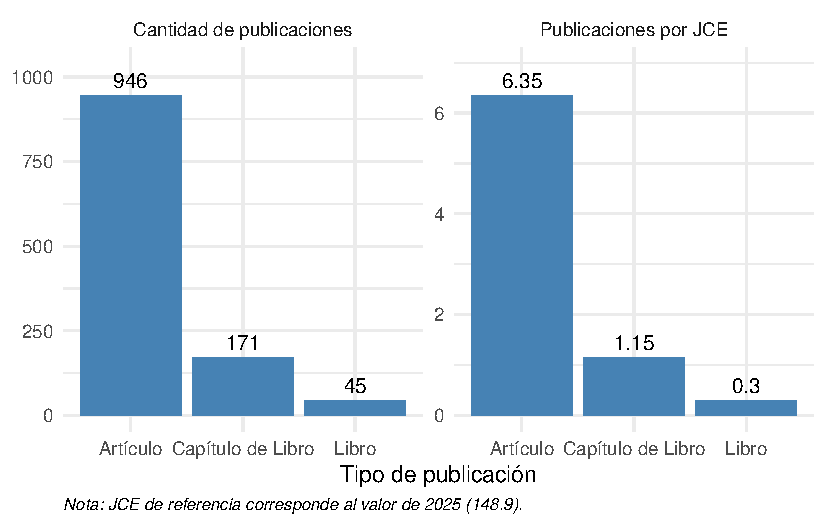
\includegraphics[keepaspectratio]{04-resultados_files/figure-pdf/fig-tipo-publicaciones-1.pdf}}

}

\end{figure}%

En el período de referencia (2020-2025), se encontraron un total de 1218
publicaciones diferentes. Entre estas, como se expone en la
Figura~\ref{fig-tipo-publicaciones}, se observa un claro dominio de la
publicación de artículos en revistas académicas (n=946), representando
un 77\% del total de publicaciones identificadas. Los capítulos de
libros en libros editados, en tanto, representan un 18\% del total,
mientras que los libros monográficos o editados son solo el 6\% del
volumen total de publicaciones. Considerando que al 31 de diciembre de
2025 la Facultad contaba con 155 Jornadas Completas Equivalente (JCE).
Esto significa que el período estudiado se registraron 7.85
publicaciones por JCE: 6.1 artículos, 1.41 capítulos de libros y 0.34
libros.

\begin{figure}

\caption{\label{fig-publicacion-anio}Publicaciones por año}

\centering{

\pandocbounded{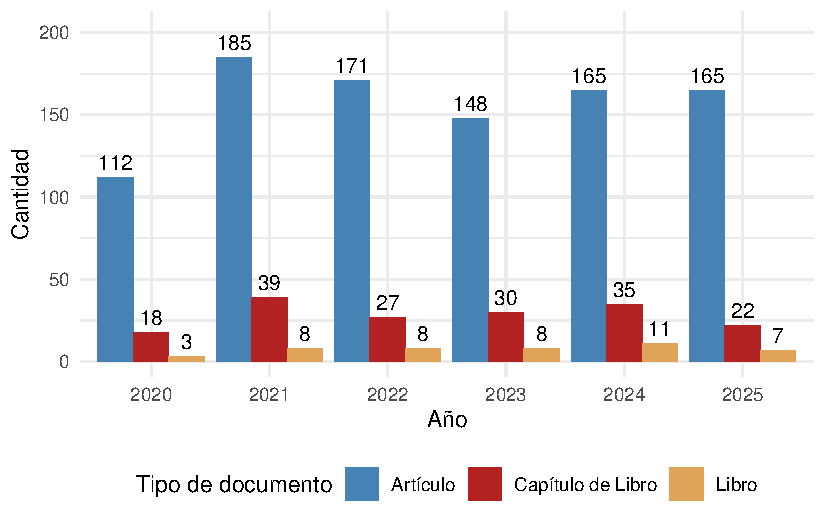
\includegraphics[keepaspectratio]{04-resultados_files/figure-pdf/fig-publicacion-anio-1.pdf}}

}

\end{figure}%

Observando la evolución por año en el período de referencia se aprecia
que entre 2020 y 2021 aumentaron la cantidad de publicaciones de manera
sustancial para los tres tipos de publicaciones analizadas. Desde ahí,
se observan fluctuaciones con relativa estabilidad. Así, los artículos
se mantienen entre 148 y 185, los capítulos de libro entre 37 y 48, y
entre 7 y 13 libros monográficos o editados.

La mediana de publicaciones por académico es de 3, con el 50\% de la
Facultad produjo entre 1 y 10 publicaciones en el período mencionado,
con máximos que llegan hasta las 50 publicaciones. La
Figura~\ref{fig-publicacion-lorenz} permite observar la concentración en
la cantidad de publicaciones entre los académicos y académicas más
productivos. Así, el 13\% de los académicos/as más productividos
concentran aproximadamente el 50\% del total de las publicaciones en el
período de referencia.

\begin{figure}

\caption{\label{fig-publicacion-lorenz}Concentración de publicaciones
por porcentaje de académicos acumulado (2020-2025)}

\centering{

\pandocbounded{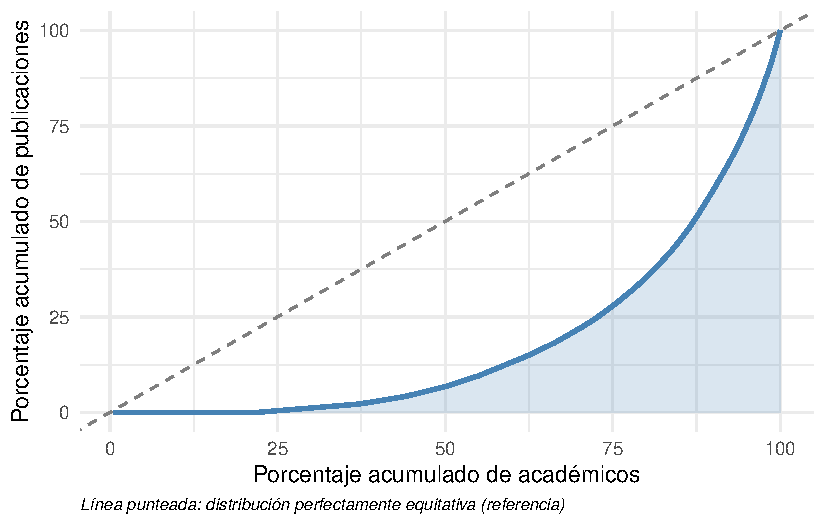
\includegraphics[keepaspectratio]{04-resultados_files/figure-pdf/fig-publicacion-lorenz-1.pdf}}

}

\end{figure}%

\subsection{Caracterización de los
autores}\label{caracterizaciuxf3n-de-los-autores}

\begin{figure}

\begin{minipage}{\linewidth}

\begin{figure}[H]

\caption{\label{fig-publicacion-depto}Publicaciones por Departamento por
JCE (2020-2025)}

\centering{

\pandocbounded{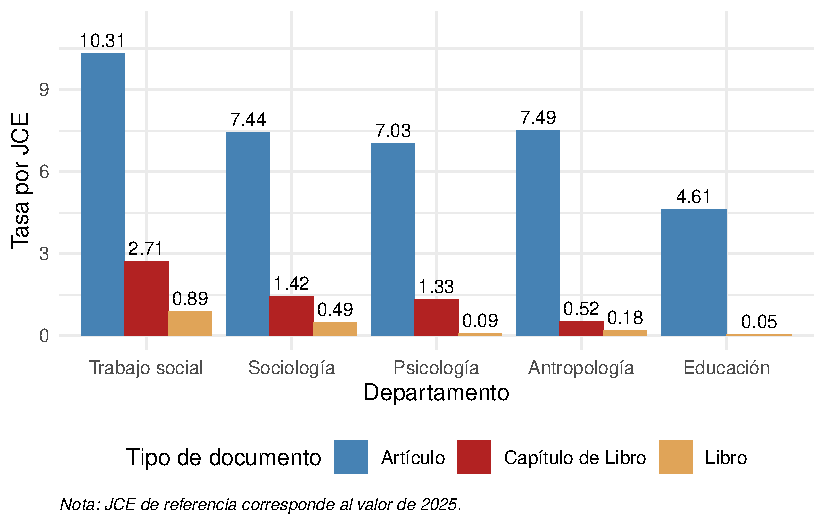
\includegraphics[keepaspectratio]{04-resultados_files/figure-pdf/fig-publicacion-depto-1.pdf}}

}

\end{figure}%

\end{minipage}%

\end{figure}%

Según se observa en el Figura~\ref{fig-publicacion-depto}, el predominio
de los artículos sobre otras formas de publicaciones es apreciable en
todos los departamentos, aunque la publicación de capítulos de libros es
superior en Trabajo Social, SOciología y Psicología. Se destaca que el
departamento de Trabajo Social es el que más publicaciones por Jornada
Completa Equivalente (2025) produce, con 14.8 publicaciones por JCE. Le
sigue el Departamento de Sociología con 9.94 publicaciones por JCE,
Psicología con 8.41, Antropología con 7.83 y Educación con 4.41.

\begin{figure}

\caption{\label{fig-publicacion-genero}Publicaciones por Género
(2020-2025)}

\centering{

\pandocbounded{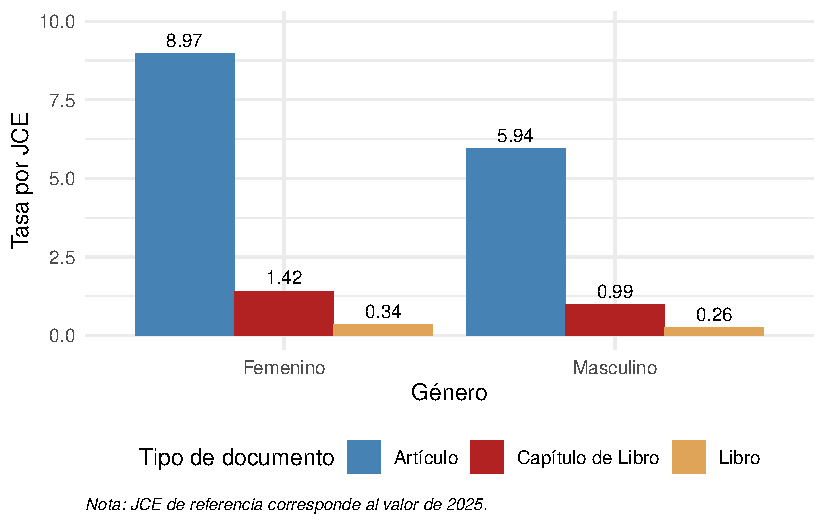
\includegraphics[keepaspectratio]{04-resultados_files/figure-pdf/fig-publicacion-genero-1.pdf}}

}

\end{figure}%

En la Figura~\ref{fig-publicacion-genero} se observa que las académicas
de la Facultad son más productivas que los académicos, completando 10.65
publicaciones por JCE en le período analizado, contra 7.32 publicaciones
por JCE entre los hombres. Aunque esta diferencia se repite en todos los
tipos de publicaciones, es más acentuada en los artículos, con una
diferencia 2.71 publicaciones por jornada completa.

\begin{figure}

\caption{\label{fig-publicacion-edad}Publicaciones por Edad y
Departamento (2020-2025)}

\centering{

\pandocbounded{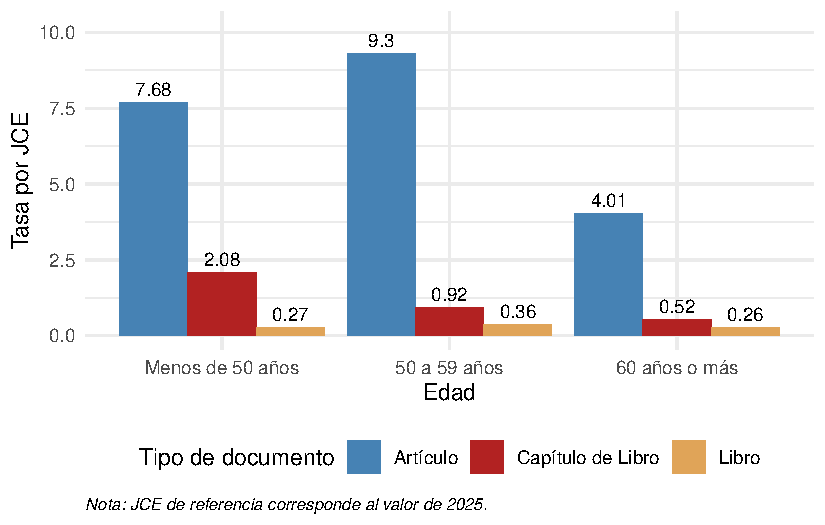
\includegraphics[keepaspectratio]{04-resultados_files/figure-pdf/fig-publicacion-edad-1.pdf}}

}

\end{figure}%

El Figura~\ref{fig-publicacion-edad} muestra que el tramo etario con
mayor productividad en el período analizado se encuentra entre los 50 y
59 años, con 10.85 publicaciones por JCE, y fuerte concentración en los
artículos. Le sigue el grupo menor de 50 años, con 9.55 publicaciones
por JCE, aunque con un menor peso relativo de los artículos en oposición
a los capítulos de libro. Mientras tanto, la productividad de los
académicos mayores de de 60 años es de 5.03 publicaciones por JCE.

\begin{figure}

\caption{\label{fig-publicacion-jerarquia}Publicaciones por Jerarquía y
Departamento (2020-2025)}

\centering{

\pandocbounded{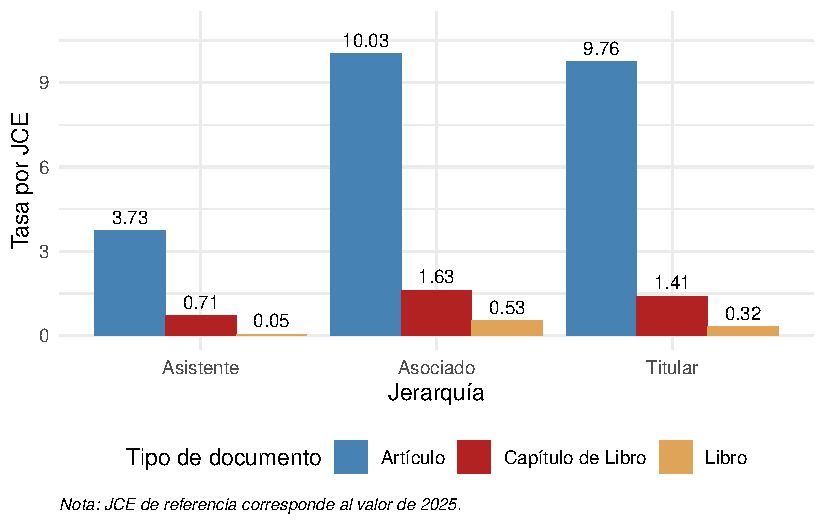
\includegraphics[keepaspectratio]{04-resultados_files/figure-pdf/fig-publicacion-jerarquia-1.pdf}}

}

\end{figure}%

LA Figura~\ref{fig-publicacion-jerarquia} muestra las diferencias por
jerarquía. Se observa que hay un salto importante entre la jerarquía de
asistente y de asociado, pasando de 4.96 publicaciones por JCE a 12.39.
La diferencia entre profesores asociados y titulares es menor, con los
primeros teniendo una mayor proporción de artículos publicados y los
segundo teniendo una mayor cantidad de publicaciones en capítulos de
libro en relación a otras jerarquías.

\section{Artículos y Revistas}\label{artuxedculos-y-revistas}

\subsection{Indexaciones}\label{indexaciones}

Los artículos de investigación representan con diferencia la mayor parte
de la producción académica de la Facultad, con 946 registros diferentes,
o un 77\% del total de las publicaciones identificadas. La
Figura~\ref{fig-index} muestra la distribución de las indexaciones de
las revistas en que publican los académicos de FACSO. De tal modo, se
observa que el 78\% de las publicaciones se encuentran en revistas
indexadas en WoS (42\%) o Scopus (36\%), posiblemente en consonancia con
los modelos de evaluación de ANID en sus fondos concursables. Más abajo
se encuentran las revistas indexadas en Scielo, con un 11\% de las
publicaciones en el período analizada. La categoría ``Otra'' agrega
revistas en indexadas en el \emph{Emerging Sources Citacion Index}
(ESCI), la \emph{European Reference Index for the Humanities and Social
Sciences} (ERIH Plus), \emph{Latindex}, el \emph{Directory of Open
Access Journals} (DOAJ), entre otras. En su conjunto, éstas acumulan el
11\% de las publicaciones totales.

\begin{figure}

\caption{\label{fig-index}Publicaciones por Indexación de la Revista
(2020-2025)}

\centering{

\pandocbounded{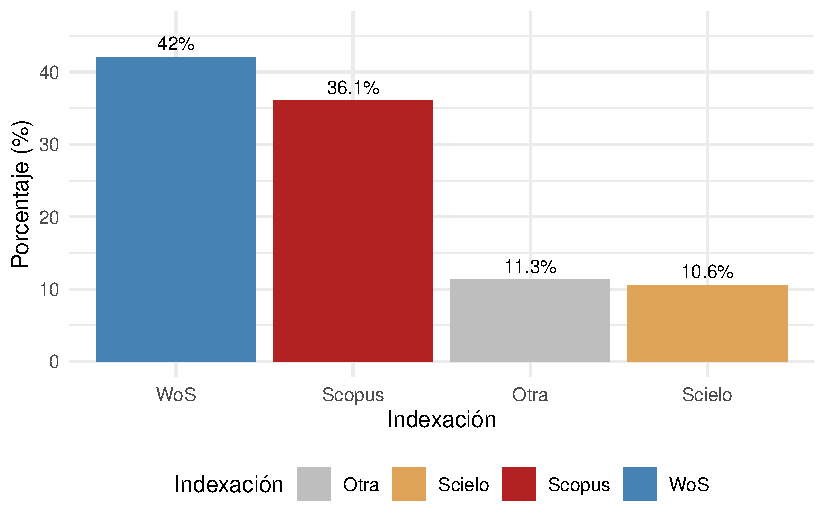
\includegraphics[keepaspectratio]{04-resultados_files/figure-pdf/fig-index-1.pdf}}

}

\end{figure}%

\begin{figure}

\caption{\label{fig-index-evolucion}Evolución de Publicaciones por
Indexación de la Revista (2020-2025)}

\centering{

\pandocbounded{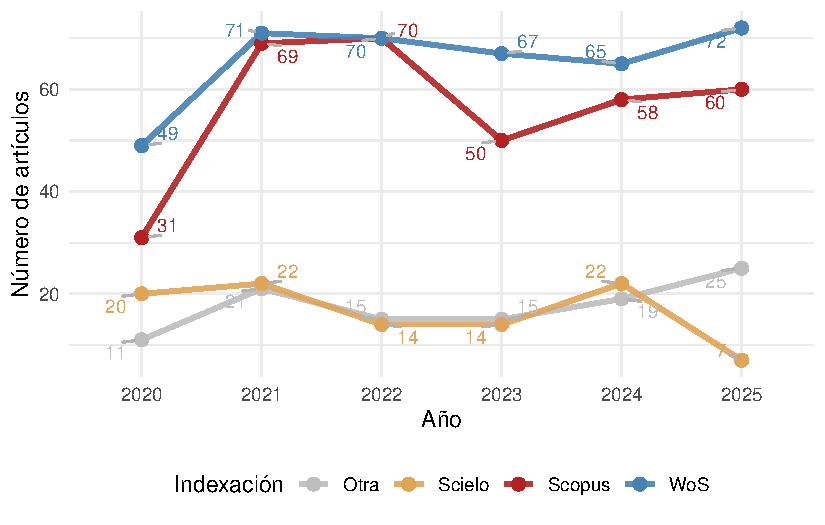
\includegraphics[keepaspectratio]{04-resultados_files/figure-pdf/fig-index-evolucion-1.pdf}}

}

\end{figure}%

La Figura~\ref{fig-index-evolucion} muestra la evolución de la cantidad
de publicaciones en cada indexación durante el período analizado. La
predominancia de WoS y Scopus se mantiene en todo los años,
particularmente tras la recuperación post-pandemia en 2021. Durante 2021
y 2022, prácticamente no hay diferencias entre ambas bases de datos. Sin
embargo, desde 2023 se abre una brecha en favor a Web of Science que ha
fluctuado entre 7 y 12 publicaciones por año. También es interesante que
las publicaciones indexadas en Scielo se habían mantenido entrw 14 y 22,
incluso en 2020 durante la pandemia, para caer bruscamente en 2025. Por
supuesto, no es posible establecer aún las causas o si esto es una
tendencia que se mantendrá en el tiempo.

\begin{figure}

\caption{\label{fig-index-depto}Publicaciones por Indexación de la
Revista por Departamento (2020-2025)}

\centering{

\pandocbounded{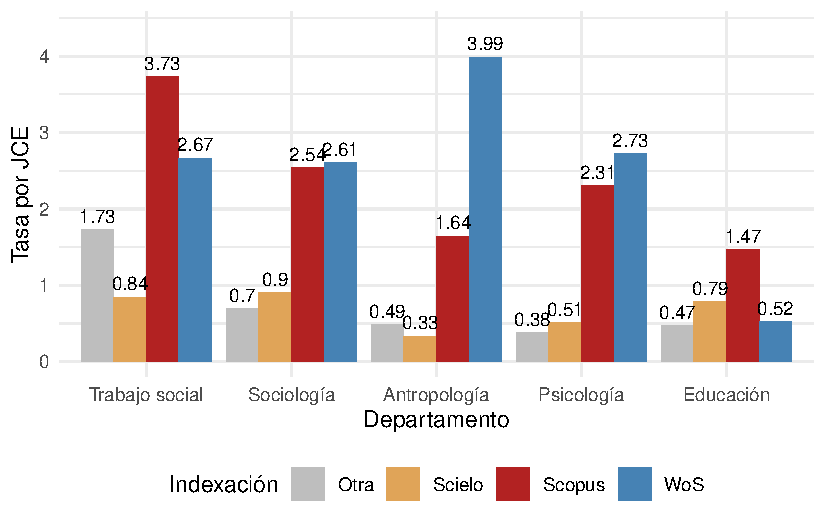
\includegraphics[keepaspectratio]{04-resultados_files/figure-pdf/fig-index-depto-1.pdf}}

}

\end{figure}%

La Figura~\ref{fig-index-depto} muestra que hay diferencias importantes
entre los departamentos. Por un lado, en Antropología predominan las
publicaciones en WoS, principalmente en revistas relaciondas a la
arqueología y la antropología física. Mientras tanto, el Departamento de
Trabajo Social muestra una mayor cantidad de publicaciones en Scopus por
JCE, al igual que el Departamento de Educación. El Departamento de
Psicología y el Departamento de Sociología, por su lado, muestran un
mayor nivel de paridad entre entre ambas bases de datos, con un leve
predominio de WoS. La Tabla~\ref{tbl-index-depto} muestra las revistas
con mayor frecuencia por departamento, reflejando las tendencias antes
mencionadas. Asimismo, se observa una fuerte presencia de la revistas de
la Facultad, tales como Enfoques Educaciones (Departamento de
Educación), Revista de Psicología (Departamento de Psicología), Última
Década y Revista de Sociología (Departamento de Sociología), y
Propuestas Críticas en Trabajo Social y Revista MAD (Departamento de
Trabajo Social).

\begin{table}

\caption{\label{tbl-index-depto}Revistas con mayor cantidad de
publicaciones por Departamento (2020-2025)}

\centering{

\centering
\begin{tabular}[t]{llr}
\toprule
Publicación & Indexación & Frecuencia\\
\midrule
\addlinespace[0.3em]
\multicolumn{3}{l}{\textbf{Antropología}}\\
\hspace{1em}CHUNGARA-REVISTA DE ANTROPOLOGIA CHILENA & WoS & 11\\
\hspace{1em}JOURNAL OF ARCHAEOLOGICAL SCIENCE-REPORTS & WoS & 8\\
\hspace{1em}ESTUDIOS ATACAMENOS & WoS & 6\\
\hspace{1em}MAGALLANIA & WoS & 6\\
\hspace{1em}QUATERNARY INTERNATIONAL & WoS & 5\\
\addlinespace[0.3em]
\multicolumn{3}{l}{\textbf{Educación}}\\
\hspace{1em}ESTUDIOS PEDAGOGICOS (VALDIVIA) & Scopus & 6\\
\hspace{1em}Revista enfoques educacionales & Scielo & 5\\
\hspace{1em}Revista de estudios y experiencias en educación & Scielo & 4\\
\hspace{1em}Dialogo andino & Scopus & 2\\
\hspace{1em}REVISTA COMPLUTENSE DE EDUCACION & Scopus & 2\\
\addlinespace[0.3em]
\multicolumn{3}{l}{\textbf{Psicología}}\\
\hspace{1em}Revista de psicología & Scielo & 10\\
\hspace{1em}Psykhe & Scopus & 8\\
\hspace{1em}PSICOPERSPECTIVAS & Scopus & 6\\
\hspace{1em}TERAPIA PSICOLOGICA & WoS & 5\\
\hspace{1em}SUSTAINABILITY & WoS & 4\\
\addlinespace[0.3em]
\multicolumn{3}{l}{\textbf{Sociología}}\\
\hspace{1em}ULTIMA DECADA & Scielo & 7\\
\hspace{1em}Revista de Sociología & Otra & 7\\
\hspace{1em}Estudios Sociologicos & Scopus & 5\\
\hspace{1em}FRONTIERS IN SOCIOLOGY & Scopus & 4\\
\hspace{1em}Revista Chilena de Derecho y Ciencia Política & Scopus & 4\\
\addlinespace[0.3em]
\multicolumn{3}{l}{\textbf{Trabajo social}}\\
\hspace{1em}Propuestas Críticas en Trabajo Social-Critical Proposals in Social Work & Otra & 24\\
\hspace{1em}REVISTA MAD-REVISTA DEL MAGISTER EN ANALISIS SISTEMICO APLICADO A LA SOCIEDAD & Scopus & 10\\
\hspace{1em}RUMBOS TS Un Espacio Crítico para la Reflexión en Ciencias Sociales & Scielo & 6\\
\hspace{1em}FRONTIERS IN PSYCHOLOGY & WoS & 4\\
\hspace{1em}SOCIAL WORK EDUCATION & Scopus & 4\\
\bottomrule
\end{tabular}

}

\end{table}%

Figura~\ref{fig-index-carac} muestra la cantidad de publicaciones por
JCE según género, edad y jerarquía de los autores. En general, se
aprecia que las tendencias observadas son las mismas, con WoS y Scopus
acaparando la mayor parte de la productividad, y la primera estando
sobre la segunda en la mayoría de los grupos analizados. También se
mantienen tendencias tales como que las mujeres
(Figura~\ref{fig-index-carac-1}) y los académicos de entre 50 y 59 años
(Figura~\ref{fig-index-carac-2}) publican más en todas las indexaciones.
Respecto a la jerarquía, como se observa en
Figura~\ref{fig-index-carac-3}, mientras los profesores titulares son
quienes más publican en WoS por JCE, los profesores asociados los
superan en Scopus y Scielo.

\begin{figure}

\caption{\label{fig-index-carac}Publicaciones por Indexación y
características de los autores}

\centering{

\subcaption{\label{fig-index-carac-1}Publicaciones por Indexación de la
Revista por Género del autor(2020-2025)}

\centering{

\pandocbounded{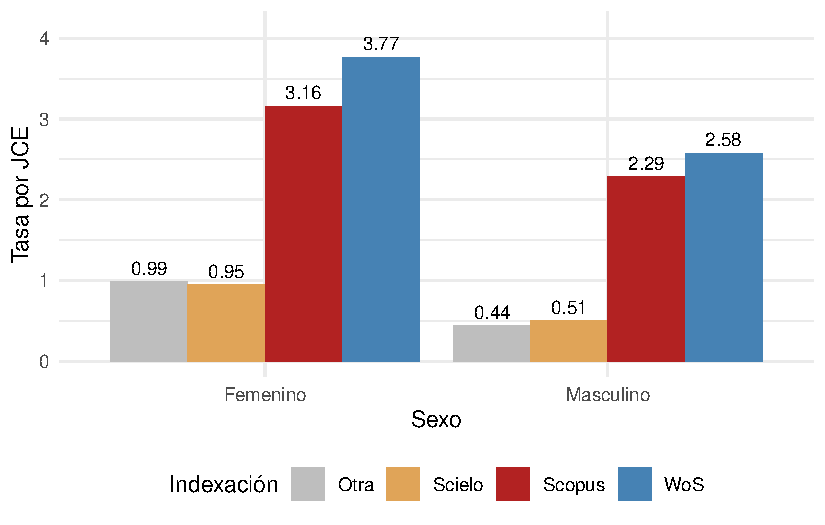
\includegraphics[keepaspectratio]{04-resultados_files/figure-pdf/fig-index-carac-1.pdf}}

}

\subcaption{\label{fig-index-carac-2}Publicaciones por Indexación de la
Revista por Edad del autor(2020-2025)}

\centering{

\pandocbounded{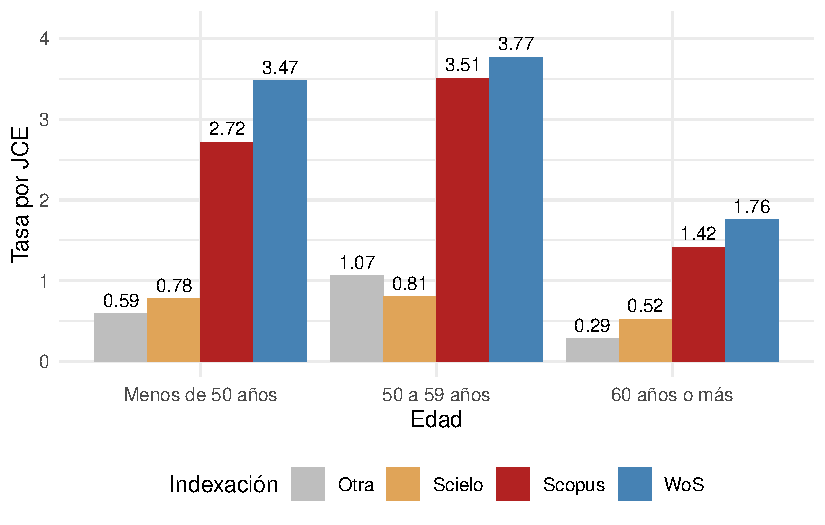
\includegraphics[keepaspectratio]{04-resultados_files/figure-pdf/fig-index-carac-2.pdf}}

}

\subcaption{\label{fig-index-carac-3}Publicaciones por Indexación de la
Revista por Jerarquia del autor(2020-2025)}

\centering{

\pandocbounded{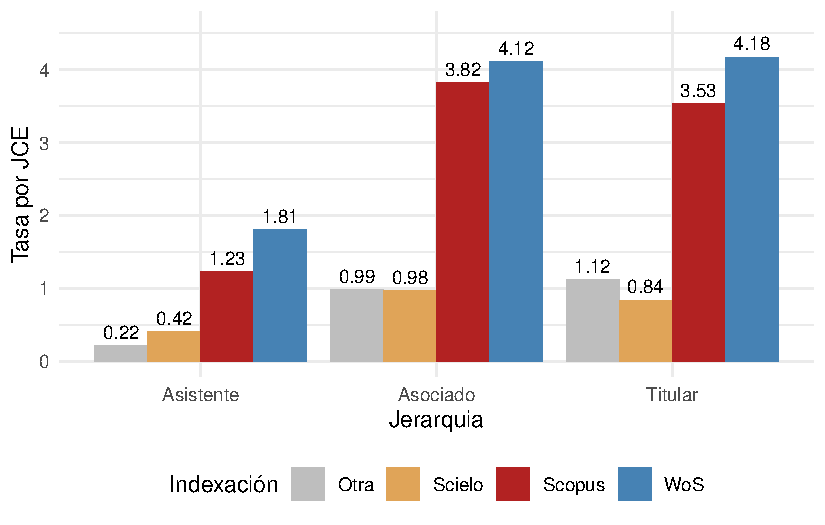
\includegraphics[keepaspectratio]{04-resultados_files/figure-pdf/fig-index-carac-3.pdf}}

}

}

\end{figure}%

\subsection{Número de Citas}\label{nuxfamero-de-citas}

A través de la API de Scopus, se encontraron registro de las citas de
674 artículos durante el período estudiado. La suma de citas entre 2020
y 2025 asciende a un total de 4854, lo que equivale a un promedio de 6.7
citas por artículos. Si se ordenan las citas de mayor a menor, es
posible observar que el índice h agregado de la institución es igual a
30. En otras palabras, entre 2020 y 2025 los académicos de la Facultad
publicaron un total de 30 artículos que registran 30 citas o más.

Ahora bien, se observa una gran dispersión en la cantidad de citas por
artículo. El rango de citas va de 0 a un máximo de 307. El artículo
mediano cuenta con 3 citaciones, con el 50\% de las publicaciones
registrando entre 1 y 7 citas. Esta amplia dispersión se observa
claramente en Figura~\ref{fig-citas-densidad}, donde se observa una
mayor proporción de artículos con 0 a 2 citas, con una cola larga hacia
la derecha que se extiende más allá de las 300 citas.

\begin{figure}

\caption{\label{fig-citas-densidad}Distribución de citas por artículos
(2020-2025)}

\centering{

\pandocbounded{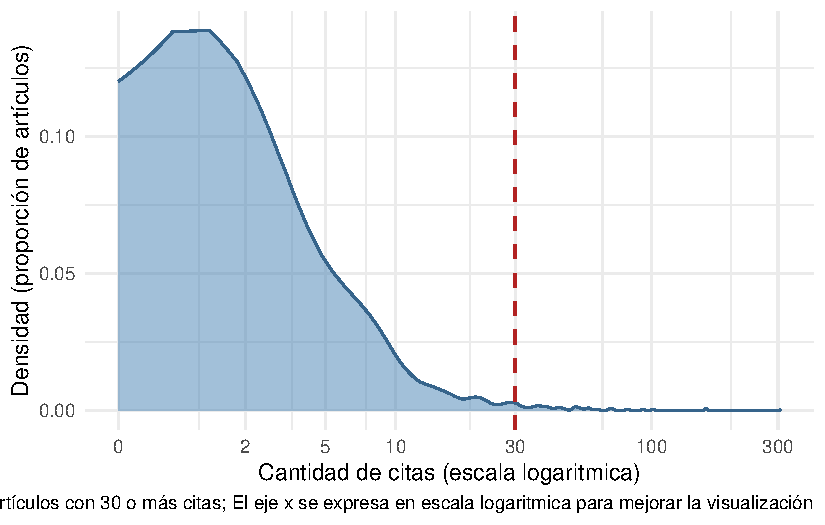
\includegraphics[keepaspectratio]{04-resultados_files/figure-pdf/fig-citas-densidad-1.pdf}}

}

\end{figure}%

La Tabla~\ref{tbl-citas-depto} muestra la cantidad de artículo, el total
de citas y el índice h para cada Departamento de la Facultad. El
departamento de Psicología tiene la mayor cantidad de citas en el
período analizado, con 2148 citas y un índice h de 22. Le siguen el
departamento de Antropología con 1169 citas y un índice h de 16; el
departamento de Sociología con 951 citas y un índice h de 15; el
departamento de Trabajo Social y el departamento de Educación con 90
citas y un índice h de 5.

\begin{longtable}[t]{lccc}

\caption{\label{tbl-citas-depto}Citas e Indíce h por Departamento
(2020-2025)}

\tabularnewline

\toprule
Departamento & Artículos & Total de citas & Índice h\\
\midrule
Antropología & 178 & 1169 & 16\\
Educación & 36 & 90 & 5\\
Psicología & 217 & 2148 & 22\\
Sociología & 134 & 951 & 15\\
Trabajo social & 139 & 774 & 12\\
\bottomrule

\end{longtable}

La Tabla~\ref{tbl-citas} permite aprecias las diferencias en la cantidad
de citas e índice h según género, edad y jerarquía académica. Se
observan tendencias similares a las que expusieron respecto al volúmen
de publicación. Las mujeres exhiben una mayor cantidad de citas y un
mayor índice h que los hombres, pese a representar una cantidad menor de
JCE en la Facultad. Los académicos entre 50 y 59 años, y auquellos con
jerarquía académica de Asociado, presentan la mayor cantidad de citas e
índice h. Cabe destacar, con todo, que la diferencia en la cantidad de
citas entre profesores asociados y titulares se explica mayormente por
la menor cantidad de académicos en la jerarquía titular.

\begin{longtable}[t]{lccc}

\caption{\label{tbl-citas}Citas e Indíce h por características de los
autores (2020-2025)}

\tabularnewline

\toprule
Categoría & Artículos & Total de citas & Índice h\\
\midrule
\addlinespace[0.3em]
\multicolumn{4}{l}{\textbf{Género}}\\
\hspace{1em}Femenino & 464 & 3566 & 26\\
\hspace{1em}Masculino & 342 & 2121 & 22\\
\addlinespace[0.3em]
\multicolumn{4}{l}{\textbf{Tramo de edad}}\\
\hspace{1em}Menos de 50 años & 271 & 1361 & 16\\
\hspace{1em}50 a 59 años & 426 & 3449 & 25\\
\hspace{1em}60 años o más & 109 & 877 & 15\\
\addlinespace[0.3em]
\multicolumn{4}{l}{\textbf{Jerarquía académica}}\\
\hspace{1em}Asistente & 153 & 792 & 12\\
\hspace{1em}Asociado & 473 & 3553 & 27\\
\hspace{1em}Titular & 178 & 1341 & 17\\
\bottomrule

\end{longtable}

\bookmarksetup{startatroot}

\chapter{Discusión}\label{discusiuxf3n}

Interpreta resultados, limitaciones y aportes.

\bookmarksetup{startatroot}

\chapter{Conclusiones}\label{conclusiones}

Síntesis y proyecciones futuras.

\bookmarksetup{startatroot}

\chapter{Referencias}\label{referencias}

\phantomsection\label{refs}
\begin{CSLReferences}{1}{0}
\bibitem[\citeproctext]{ref-bourdieu2012}
Bourdieu, P. (2012). \emph{La distinci{ó}n: Criterio y bases sociales
del gusto}. Taurus.

\bibitem[\citeproctext]{ref-desmond2019poverty}
Desmond, M., \& Wilmers, N. (2019). The Racialized Geography of Housing.
\emph{American Journal of Sociology}.

\bibitem[\citeproctext]{ref-xie2017bookdown}
Xie, Y. (2017). \emph{bookdown: Authoring Books and Technical Documents
with R Markdown}. Chapman; Hall/CRC.

\end{CSLReferences}


\backmatter

% --- Cuerpo del libro (capítulos) en arábigos ---
\mainmatter
\pagestyle{scrheadings}

% --- (Opcional) Estilo del índice general ---
% \addtocontents{toc}{\protect\thispagestyle{plain}}


\end{document}
